Consta de dos clases \textbf{Numero} y \textbf{Tarjeta} las cuales ambas se definen en tarjeta.hpp y se implementan en tarjeta.cpp.

\subsection{Clase Numero}
Un Numero contendrá un atributo de tipo Cadena, ya que este «número» puede tener espacios de separación al principio, al final o, más normal, en medio.

Su constructor recibirá como parámetro esa Cadena con el número. Tendrá que quitarle los blancos y comprobar que es un número válido. Si no lo fuera lanzará la excepción \textbf{Numero::Incorrecto}.
Para saber si un dígito de dicho número es un caracter en blanco, recorreremos el número entero y mediante \texttt{isspace()}.

Dentro de la clase Numero vamos a declarar Razon con los elementos LONGITUD, DIGITOS y NO\_VALIDO, para representar por qué un Numero no es válido, y la clase Incorrecto, con un atributo de tipo \texttt{Numero::Razon}, el constructor que recibe una Razon como parámetro, y el método observador \textbf{razon()} que devuelve el atributo.

También contendrá un operadore de conversión a cadena de caracteres de bajo nivel, y deberá definirse el operador «menor que» para dos objetos de la clase.
\newpage
\subsection{Clase Tarjeta}
En la clase Tarjeta vamos a encontrar un tipo enum para indicar el tipo de la tarjeta, siendo las opciones: Otro, VISA, Mastercard, Maestro, JCB y AmericanExpress.

Tendrá varios atributos como:

\begin{itemize}
    \item Un Numero constante, que es el número de la tarjeta que viene troquelado,
    \item Un puntero a Usuario, que es el titular,
    \item Un Fecha constante, que es la de cadudidad,
    \item Un booleano que indicará si la Tarjeta está o no activa, siempre se crea activa.
\end{itemize}

La Tarjeta se construirá solamente a partir del Numero, el Usuario y la Fecha de cadudidad. Esta última es importante debido a que vamos a declarar la clase de excepción \textbf{Tarjeta::Caducada}.


Esta clase de excepción tendrá un atributo que almacena la fecha caducada, un constructor que la reciba como parámetro observador \texttt{cuando()}, que lo devolverá. 

En el constructor vamos a crear la asociación entre Tarjeta y Usuario mediante el método \texttt{es\_titular\_de()}.

También vamos a declara una clase de excepción \textbf{Tarjeta::Num\_Duplicado}, debido a que no pueden haber dos Tarjetas con el mismo número. Esta clase de excepción tiene un atributo que es el Numero, y un método observador \texttt{que()} que lo devuelve.

Vamos a eliminar tanto el \textbf{constructor de copia} como el \textbf{operador de asignación por copia}, debido a que no se puede crear una Tarjeta que tenga los mismo atributos que otra.

Vamos a tener varios métodos observador que van a devolver los atributos de la Tarjeta, estos métodos serán: \texttt{numero()}, \texttt{titular()}, \texttt{caducidad()} y \texttt{activa()}, este último se sobrecargará que recibirá el nuevo estádo de la Tarjeta en un parámetro booleano y devolverá dicho estado.

Además vamos a tener el método observador \texttt{tipo()} devolverá el Tipo de la Tarjeta. El tipo de Tarjeta estará determinado por los primeros dígitos del Numero que la contiene:
\begin{itemize}
    \item \textbf{AmericanExpress:} Los dos primeros dígitos del Numero son 34 ó 37.
    \item \textbf{JCB:} El primer dígito es 3 a excepción de 34 o 37.
    \item \textbf{VISA:} El primer dígito es 4.
    \item \textbf{Mastercard:} El primer dígito es 5.
    \item \textbf{Maestro:} El primer dígito es 6.
    \item \textbf{Otro:} El cualquier otro dígito.
\end{itemize}

Cuando se detruya un Usuario, como las tarjetas no se destruyen segurían ``vivas'' pero sin ningún titular asociado, por tanto, se llamará al método \texttt{anula\_titular()} que dará al puntero que representa al titular el valor nulo y desactivará la Tarjeta poniendo a \textbf{false} el atributo correspondiente, es decir, activa pasa a falso. El destructor de la clase Usuario llamará a este método para cada una de sus tarjetas.

A la hora de destruir una Tarjeta, en el destructor tenemos que eliminar la relación entre Tarjeta y Usuario, para ello llamamos al método \textbf{Usuario::no\_es\_titular\_de()} sobre su titular, en caso de que este no haya sido destruido previamente; de lo contrario, la Tarjeta habrá sido desligada de su Usuario al ser destruido este (vea el punto anterior).

Vamos a sobrecargar el operador de inserción en flujo \texttt{\textbf{operator <<}} para mostrar los atributos de la clase Tarjeta siguiendo el formato:

\begin{figure}[h]
    \begin{minipage}{0.4\textwidth}
            \texttt{tipo tarjeta}\\
            \texttt{ numero tarjeta}\\
            \texttt{titular facial}\\
            \texttt{Caduca: MM/AA}
    \end{minipage}
    \hfill
    \begin{minipage}{0.5\textwidth}
        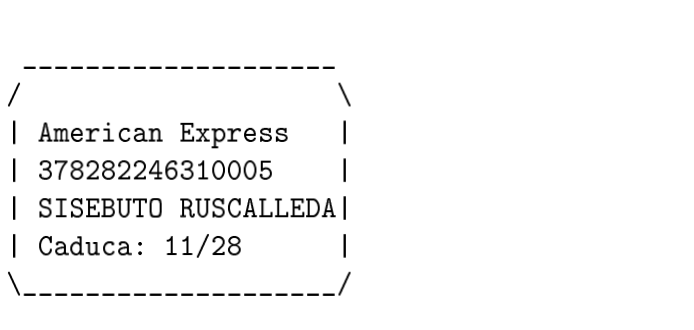
\includegraphics[width=\textwidth]{Pics/P2_2.png}
    \end{minipage}
    Donde MM es el mes de la fecha de caducidad, expresado con dos dígitos y AA son los dos últimos dígitos del año; por ejemplo: 11/28 sería noviembre de 2028.
    
    El titular facial es el nombre y apellido concatenados en mayúsculas del usuario titular de la tarjeta.

    Las lineas del formato no hace falta que las implementes, es más por estética.
\end{figure}
Para imprimir el nombre del tipo de la tarjeta (VISA, American Express...), deberá
sobrecargar también el operador de inserción para \textbf{Tarjeta::Tipo}, el cual imprimirá el texto «Tipo indeterminado» cuando el valor sea \textbf{Tipo::Otro}.

Dos Tarjeta podrán ordenarse por sus números. Para ello Tendrá que definir el operador menor-que de dos tarjetas.

\subsubsection{Tarjeta.hpp}
\begin{minted}[breaklines]{C++}
#ifndef TARJETA_HPP
#define TARJETA_HPP

//Inclusión de librerias
#include "../P1/fecha.hpp"
#include "../P1/cadena.hpp"
#include "usuario.hpp"
#include <iostream>
#include <set>
#include <algorithm> //remove_if
#include <cctype> //isspace
#include <cstring>
//declaraciones adelantadas
class Usuario;
class Clave;

/*-----Clase Numero-----*/
class Numero{
public:
    //tipos de excepciones
    typedef enum {LONGITUD,DIGITOS,NO_VALIDO}Razon;
    Numero(const Cadena&);
    
    //operador de conversion a const char*
    inline operator const char*()const{return numero_.operator const char *();}
    //sobrecarga del operador < para comparar numeros
    friend bool operator < (const Numero&, const Numero&);
    //clase de la excepcion
    class Incorrecto{
        Razon razon_;
        public:
            Incorrecto(const Razon& r):razon_(r){};
            const Razon& razon()const{return razon_;}
    };

private:
    Cadena numero_;
    //metodos extras para el constructor
    Cadena eliminar_espacios(const Cadena&); //devuelve la cadena sin espacios
    Cadena longitud(const Cadena&); //comprueba la longitud de la cadena es correcta o no
};

/*-----Clase Tarjeta-----*/
class Tarjeta{
public:
    //tipos de tarjetas
    typedef enum {Otro,VISA,Mastercard,Maestro,JCB,AmericanExpress} Tipo;
    Tarjeta(const Numero&, Usuario&, const Fecha&);
    //no se pueden crear tarjetas por copia de otras
    Tarjeta(const Tarjeta&)=delete;
    Tarjeta operator =(const Tarjeta&)=delete;
    //Observadores de la clase
    const Numero& numero()const noexcept{return numero_;}
    const Usuario* titular()const noexcept{return titular_;}
    const Fecha& caducidad()const noexcept{return caducidad_;}
    bool activa()const noexcept{return activa_;}
    bool activa(bool estado) noexcept {activa_=estado;return activa_;}//version modificadora de la anterior
    Tipo tipo()const noexcept;

    //destructor de la clase
    ~Tarjeta();
    //Clase de la excepcion tarjeta caducada
    class Caducada{
        Fecha fecha_;
        public:
            Caducada(const Fecha fecha):fecha_(fecha){};
            const Fecha& cuando()const{return fecha_;}
    };
    //Clase de la excepcion tarjeta duplicada
    class Num_duplicado{
        Numero num_;
        public:
            Num_duplicado(const Numero& num):num_(num){};
            const Numero& que()const{return num_;}
    };
    //Clase de la excepcion tarjeta desactivada
    class Desactivada{};
private:
    const Numero numero_;
    Usuario* const titular_;
    const Fecha caducidad_;
    bool activa_;

    //método privado de la clase
    //hacemos que la clase usuario sea amiga para poder hacer uso de este método
    friend class Usuario;
    void anula_titular();

    //conjunto de tarjetas
    static std::set<Numero>tarjetas_;
};
std::ostream& operator <<(std::ostream&, const Tarjeta& )noexcept;
std::ostream& operator <<(std::ostream&, const Tarjeta::Tipo& )noexcept;
//sobrecarga del operador <, para ordenar tarjetas
bool operator <(const Tarjeta&,const Tarjeta&);
#endif // !TARJETA_HPP
\end{minted}

\subsubsection{Tarjeta.cpp}
\begin{minted}[breaklines]{C++}
#include "tarjeta.hpp"
//inicialización del conjunto estático de tarjetas
std::set<Numero> Tarjeta::tarjetas_;
//Hacemos uso del algoritmo de luhn para ver si el numero de la tarjeta es correcto o no
bool luhn(const Cadena& numero);
/*-----Clase Numero-----*/
Numero::Numero(const Cadena& numero):numero_(longitud(numero)){
    char caracteres[] = "abcdefghijklmnopqrstuvwxyzABCDEFGHIJKLMNOPQRSTUVWXYZ./";
    //Comprobamos que está en el rango de caracteres
    if(strcspn(numero_.operator const char *(),caracteres)<numero_.length())
        throw Incorrecto(Razon::DIGITOS);
    //comprobamos que sea correcto
    if(!luhn(numero_))throw Incorrecto(Razon::NO_VALIDO);
}
bool operator < (const Numero& a, const Numero& b){
    return strcmp(a,b)<0;
}

//metodos privados de la clase
Cadena Numero::eliminar_espacios(const Cadena& cadena){
    //creamos una cadena nueva como copia de la introducida
    Cadena aux(cadena);
    const char* original = cadena.operator const char *();
    int j =0;
    for(size_t i =0; i!=strlen(original); i++){
        if(!isspace(original[i])){
            aux[j++] = original[i];
        }
    }
    aux[j] = '\0';
    return Cadena(aux.operator const char *());
}
Cadena Numero::longitud(const Cadena& cadena){
    //creamos una cadena como copia de la introducida para calcular la longitud sin espacios
    Cadena aux = eliminar_espacios(cadena);
    if(aux.length()> 19 || aux.length() < 13 || aux.length() <= 0)
        throw Incorrecto(Razon::LONGITUD);
    return aux;
}

/*-----Clase Tarjeta-----*/
Tarjeta::Tarjeta(const Numero& numero,  Usuario& titular, const Fecha& caducidad):
    numero_(numero),titular_(&titular),caducidad_(caducidad),activa_(true){
    if(caducidad_ < Fecha())throw Caducada(caducidad_); //caducada¿?
    //Comprobamos que la tarjeta no está registrada
    if(!tarjetas_.insert(numero).second)throw Num_duplicado(numero);
    //No caducada y numero correcto -> se asigna al usuario
    titular_ -> es_titular_de(*this);
}
Tarjeta::Tipo Tarjeta::tipo()const noexcept{
    switch (numero_[0]){
    case '3':
        if(numero_[1]=='4' || numero_[1]=='7') return Tipo::AmericanExpress;
        else return Tipo::JCB;
        break;
    case '4': return Tipo::VISA; break;
    case '5': return Tipo::Mastercard; break;
    case '6': return Tipo::Maestro; break;
    default: return Tipo::Otro; break;
    }
}

Tarjeta::~Tarjeta(){
    //Para poder eliminar una tarjeta, primero debemos de desvincularla de su titular
    if(Usuario* user = const_cast<Usuario*>(titular_)) user->no_es_titular_de(*this);
    tarjetas_.erase(numero_); //eliminamos despues de desvincular
}

bool operator <(const Tarjeta& a,const Tarjeta& b){
    return a.numero() < b.numero();
}

std::ostream& operator <<(std::ostream& output, const Tarjeta& t)noexcept{
    //primero tenemos que concatenar el nombre y el apellido del titular
    Cadena nombre_apell = t.titular()->nombre() + " " + t.titular()->apellidos();
    //las tenemos que imprimir en mayusculas
    int i =0;
    while(nombre_apell[i]!='\0'){
        if(islower(nombre_apell[i]))
            nombre_apell[i]=toupper(nombre_apell[i]);
        i++;
    }
    output<<std::setw(2)<<std::setfill(' ')<<' '<<t.tipo()
    <<std::setw(2)<<std::setfill(' ')<<' '<<t.numero()<<"\n"
    <<std::setw(2)<<std::setfill(' ')<<' '<<nombre_apell<<"\n"
    <<std::setw(2)<<std::setfill(' ')<<' '<<"Caduca: "<<std::setfill('0')<<std::setw(2)<<t.caducidad().mes()
    <<"/"<<std::setw(2)<<(t.caducidad().anno() % 100)<<std::endl;
    return output;
}

std::ostream& operator <<(std::ostream&output, const Tarjeta::Tipo& tipo )noexcept{
    switch (tipo){
    case Tarjeta::Otro: output<<"Otro"<<std::endl; break;
    case Tarjeta::VISA: output<<"VISA"<<std::endl; break;
    case Tarjeta::Mastercard: output<<"Mastercard"<<std::endl;break;
    case Tarjeta::Maestro: output<<"Maestro"<<std::endl; break;
    case Tarjeta::JCB: output<<"JCB"<<std::endl; break;
    case Tarjeta::AmericanExpress: output<<"AmericanExpress"<<std::endl; break;
    default: output<<"Otra"<<std::endl;break;
    }
return output;
}
void Tarjeta::anula_titular(){
    (Usuario*&) titular_=nullptr;
    activa_=false;
}
\end{minted}